% (c) 2012-2013 Claudio Carboncini - claudio.carboncini@gmail.com
% (c) 2012-2014 Dimitrios Vrettos - d.vrettos@gmail.com

\section{Esercizi}

%\subsection{Esercizi dei singoli paragrafi}

%\subsubsection*{18.2 - Equazioni numeriche frazionarie}

\begin{esercizio}[\Ast]
\label{ese:18.1}
Risolvi le seguenti equazioni frazionarie.
\begin{multicols}{2}
\begin{enumeratea}
 \item $\dfrac{2}{x+1}=\dfrac{1}{x+2}$;
 \item $\dfrac{1}{x-1}=2$;
 \item $1-\dfrac{1}{x+1}=0$;
 \item $\dfrac{2x-4}{x-2}=0$.
\end{enumeratea}
\end{multicols}
\end{esercizio}

\begin{esercizio}[\Ast]
\label{ese:18.2}
Risolvi le seguenti equazioni frazionarie.
\begin{multicols}{2}
\begin{enumeratea}
 \item $\dfrac{x}{x+1}-\dfrac{1}{x-1}=1$;
 \item $\dfrac{1}{x-3}=\dfrac{x}{3-x}$;
 \item $\dfrac{x-1}{x^{2}-4}=-{\dfrac{5}{x+2}}$;
 \item $\dfrac{3}{x+1}=\dfrac{2}{x+1}$.
\end{enumeratea}
\end{multicols}
\end{esercizio}
%\newpage
\begin{esercizio}[\Ast]
\label{ese:18.3}
Risolvi le seguenti equazioni frazionarie.
\begin{multicols}{2}
\begin{enumeratea}
 \item $\dfrac{1}{3-x}-\dfrac{4}{2x-6}=0$;
 \item $\dfrac{x^{2}-1}{x-1}+x=2x+1$;
 \item $\dfrac{x}{x^{2}-4}=\dfrac{1}{x+2}$;
 \item $\dfrac{1}{x}-\dfrac{3}{x^{2}}=\dfrac{2-2x}{x^{3}}$.
\end{enumeratea}
\end{multicols}
\end{esercizio}

\begin{esercizio}[\Ast]
\label{ese:18.4}
Risolvi le seguenti equazioni frazionarie.
\begin{multicols}{2}
\begin{enumeratea}
 \item $\dfrac{x-2}{x-1}=\dfrac{x-1}{x-2}$;
 \item $\dfrac{x+3}{x+1}=x+3$;
 \item $\dfrac{3x+1}{3x^{2}+x}=1$;
 \item $\dfrac{6+x}{x-3}=\dfrac{x^{2}}{x-3}$.
\end{enumeratea}
\end{multicols}
\end{esercizio}

\begin{esercizio}[\Ast]
\label{ese:18.5}
Risolvi le seguenti equazioni frazionarie.
\begin{multicols}{2}
\begin{enumeratea}
 \item $\dfrac{1}{x-2}+\dfrac{2}{x+1}=\dfrac{3}{x^{2}-x-2}$;
 \item $\dfrac{5}{x-2}-\dfrac{6}{x+1}=\dfrac{3x-1}{x^{2}-x-2}$;
 \item $\dfrac{1}{1-x}-\dfrac{x}{x-1}=0$;
 \item $\dfrac{x+1}{x-1}-\dfrac{x}{1+x}=0$.
\end{enumeratea}
\end{multicols}
\end{esercizio}

\begin{esercizio}[\Ast]
\label{ese:18.6}
Risolvi le seguenti equazioni frazionarie.
\begin{multicols}{2}
\begin{enumeratea}
 \item $\dfrac{2x+1}{2x-1}+\dfrac{4x^{2}+1}{4x^{2}-1}=2$;
 \item $\dfrac{1}{x-1}+\dfrac{2}{x}+\dfrac{1}{x^{2}-x}=0$;
 \item $\dfrac{x-1}{x^{2}-2x+1}=\dfrac{2}{2-2x}$;
 \item $4-x^{2}=\dfrac{x^{2}+5x+6}{x+2}-1$.
\end{enumeratea}
\end{multicols}
\end{esercizio}

\begin{esercizio}[\Ast]
\label{ese:18.7}
Risolvi le seguenti equazioni frazionarie.
\begin{multicols}{2}
\begin{enumeratea}
 \item $\dfrac{5}{5x+1}+\dfrac{2}{2x-1}=\dfrac{1}{1-2x}$;
 \item $\dfrac{1}{x-2}+\dfrac{2}{x+1}=\dfrac{3}{x^{2}-x-2}$;
 \item $\dfrac{30}{x^{2}-25}+\dfrac{3}{5-x}=0$;
 \item $1+\dfrac{x-1}{x+1}=\dfrac{1}{x-2}+\dfrac{1-x^{2}}{x^{2}-x-2}$.
\end{enumeratea}
\end{multicols}
\end{esercizio}
\pagebreak

\begin{esercizio}[\Ast]
\label{ese:18.8}
Risolvi le seguenti equazioni frazionarie.
\begin{multicols}{2}
\begin{enumeratea}
 \item $-{\dfrac{3x}{6-2x}}+\dfrac{5x}{10-5x}=\dfrac{1-x}{4-2x}$;
 \item $\dfrac{18x^{2}-9x-45}{4-36x^{2}}-\dfrac{6x+1}{9x-3}+\dfrac{21x-1}{18x+6}=0$;
 \item $\dfrac{1}{x+3}-\dfrac{1}{2-x}=\dfrac{x+3}{x^{2}+x-6}$;
 \item $\dfrac{1+2x}{1-2x}+\dfrac{1-2x}{1+2x}=\dfrac{6-8x^{2}}{1-4x^{2}}$.
\end{enumeratea}
\end{multicols}
\end{esercizio}

\begin{esercizio}[\Ast]
\label{ese:18.9}
Risolvi le seguenti equazioni frazionarie.
\begin{multicols}{2}
\begin{enumeratea}
 \item $\dfrac{3x}{x-2}+\dfrac{6x}{x^{2}-4x+4}=\dfrac{3x^{2}}{(x-2)^{2}}$;
 \item $(4x+6)\left(\dfrac{4}{x+1}-\dfrac{1}{x-1}\right)=0$;
 \item $\dfrac{5x}{3x^{2}-18x+15}-\dfrac{2}{3x-3}=\dfrac{5}{18x-90}$;
 \item $(x-4)(x+3)=\dfrac{(x-4)(x+3)}{x-2}$.
\end{enumeratea}
\end{multicols}
\end{esercizio}

\begin{esercizio}[\Ast]
\label{ese:18.10}
Risolvi le seguenti equazioni frazionarie.
\begin{multicols}{2}
\begin{enumeratea}
 \item $\dfrac{1}{3x+2}-\dfrac{3}{2-x}=\dfrac{10x+4}{3x^{2}-4x-4}$;
 \item $\dfrac{2x+1}{x+3}+\dfrac{1}{x-4}=\dfrac{4x-9}{x^{2}-x-12}$;
 \item $\dfrac{1}{x-1}-\dfrac{1}{x}=\dfrac{(x+1)^{2}}{2(x^{2}-1)}+1$;
 \item $\dfrac{x^{2}-1}{x+1}-\dfrac{1}{x+2}=\dfrac{x+1}{x+2}-x$.
\end{enumeratea}
\end{multicols}
\end{esercizio}

\begin{esercizio}[\Ast]
\label{ese:18.11}
Risolvi le seguenti equazioni frazionarie.
\begin{multicols}{2}
\begin{enumeratea}
 \item $\dfrac{2x+1}{1-x}+\dfrac{4x}{3+2x}=0$;
 \item $\dfrac{2+x}{2-x}-\dfrac{2-x}{2+x}+\dfrac{16}{4-x^{2}}=0$;
 \item $\dfrac{1+2x}{1-x}-\dfrac{2}{x-4}=\dfrac{3-2x}{x-4}$;
 \item $\dfrac{x-11}{2x-10}+1=\dfrac{1+2x}{3x-15}$.
\end{enumeratea}
\end{multicols}
\end{esercizio}

\begin{esercizio}[\Ast]
\label{ese:18.12}
Risolvi le seguenti equazioni frazionarie.
\begin{multicols}{2}
\begin{enumeratea}
 \item $\dfrac{5x}{x^{2}-9}+\dfrac{x-3}{x+3}=\dfrac{x+3}{x-3}$;
 \item $\dfrac{4x}{4-2x}+\dfrac{2x}{x-2}+\dfrac{1}{x+1}=\dfrac{8}{x+1}$;
 \item $\dfrac{2-x}{x+1}+\dfrac{x^{2}}{x^{2}-x-2}=-\dfrac{6}{x^{2}-x-2}+\dfrac{3}{x-2}$;
 \item $\dfrac{1}{3(x-2)}=\dfrac{x-1}{x^{2}-2x}-\dfrac{3}{4x}$.
\end{enumeratea}
\end{multicols}
\end{esercizio}

\begin{esercizio}[\Ast]
\label{ese:18.13}
Risolvi le seguenti equazioni frazionarie.
\begin{multicols}{2}
\begin{enumeratea}
 \item $\dfrac{1}{x+3}-\dfrac{2}{x+2}=\dfrac{3x-6}{x^{2}+5x+6}$;
 \item $\dfrac{2x-3}{x+2}+\dfrac{1}{x-4}=\dfrac{2}{x^{2}-2x-8}$;
 \item $\dfrac{x-1}{x+2}-\dfrac{x+2}{x-1}=\dfrac{1}{x^{2}+x-2}$;
 \item $\dfrac{3}{x-1}+\dfrac{1}{x+1}=\dfrac{12-x}{x^{2}-1}$.
\end{enumeratea}
\end{multicols}
\end{esercizio}

\begin{esercizio}[\Ast]
\label{ese:18.14}
Risolvi le seguenti equazioni frazionarie.
\begin{multicols}{2}
\begin{enumeratea}
 \item $\dfrac{1}{2} \left(x-\dfrac{1}{x}\right)-2\left(1-\dfrac{1}{x}\right)=\dfrac{x^{2}-1}{x}$;
 \item $\left(40-10x^{2}\right)^{3} \left(\dfrac{3x-1}{x+2}-\dfrac{3x}{x+1}\right)=0$;
 \item $\dfrac{x}{2x+1}+\dfrac{x+1}{2(x+2)}=\dfrac{x-1}{2x^{2}+5x+2}$;
 \item $\dfrac{3x+1}{x^{2}-9}+\dfrac{2}{3x^{2}-9x}=\dfrac{3}{x+3}$.
\end{enumeratea}
\end{multicols}
\end{esercizio}

\begin{esercizio}[\Ast]
\label{ese:18.15}
Risolvi le seguenti equazioni frazionarie.
\begin{multicols}{2}
\begin{enumeratea}
 \item $\dfrac{3(2x-3)}{x^{3}+27}+\dfrac{1}{x+3}=\dfrac{x}{x^{2}-3x+9}$;
 \item $\dfrac{1}{x^{2}-3x+2}+\dfrac{2}{x-1}=0$;
 \item $\dfrac{2x-1}{3x^{2}-75}-\dfrac{3-x}{x+5}+\dfrac{x-3}{10-2x}=\dfrac{7}{25-x^{2}}$;
 \item $\dfrac{x+2}{(x-3)^{2}}-\dfrac{1}{x-3}=\dfrac{4}{9-3x}$.
\end{enumeratea}
\end{multicols}
\end{esercizio}

\begin{esercizio}[\Ast]
\label{ese:18.16}
Risolvi le seguenti equazioni frazionarie.
\begin{enumeratea}
 \item $\left(\dfrac{x+2}{x-2}-\dfrac{x-2}{x+2}\right):\left(1+\dfrac{x+2}{x-2}\right)=\dfrac{2}{x-2}$;
 \item $\left(\dfrac{x-1}{x+1}-\dfrac{x+1}{x-1}\right):\left(1+\dfrac{x+1}{x-1}\right)+\dfrac{1}{2}=0$;
 \item $\dfrac{x^{2}}{(x-2)^{2}}=\dfrac{2}{x-2}-\dfrac{x}{(x-2)^{2}}$;
 \item $\dfrac{2x-4}{(x-1)^{2}}-\dfrac{9}{x^{3}-2x^{2}+x}=\dfrac{1}{x}\left[2+\left(\dfrac{2x-1}{1-x}\right)^{2}\right]$.
\end{enumeratea}
\end{esercizio}

\begin{esercizio}[\Ast]
\label{ese:18.17}
Risolvi le seguenti equazioni frazionarie.
\begin{enumeratea}
 \item $\dfrac{4x+3}{20}+\dfrac{7+3x^{2}}{10(x-1)}=\dfrac{3-2x}{2(x-1)}+\dfrac{x^{2}-4x+4}{2(x-1)}$;
 \item $\dfrac{x}{x^{2}+x+1}+\dfrac{1}{x-1}=\dfrac{x(2x+3)}{x^{3}-1}$;
 \item $\dfrac{3x}{x^{2}-3x}-\dfrac{x+2}{x^{2}-3x}+\dfrac{28}{5\left(x^{2}-9\right)}=\dfrac{2x}{x^{2}-9}$;
 \item $\dfrac{3}{x-2}-\dfrac{5}{x-1}+\dfrac{7}{x-3}=\dfrac{5x^{2}}{(x-1)\left(x^{2}-5x+6\right)}$.
\end{enumeratea}
\end{esercizio}

\begin{esercizio}[\Ast]
\label{ese:18.18}
Risolvi le seguenti equazioni frazionarie.
\begin{enumeratea}
 \item $\left(\dfrac{1}{x+5}-\dfrac{1}{5}\right):\left(\dfrac{1}{x-5}+\dfrac{1}{5}\right)+\dfrac{x^{2}}{x^{2}-5x}=0$;
 \item $\dfrac{1+2x}{x^{2}+2x}+\dfrac{x^{3}-6x+1}{x^{2}-4}=\dfrac{x^{2}-2x}{x-2}+\dfrac{1}{x^{2}-2x}$.
 \item $\left(1-\dfrac{1}{2}x\right):\left(1+\dfrac{1}{2}x\right)=\dfrac{2x+1}{6x+3}-\dfrac{1}{2}x+\dfrac{x^{2}}{2x+4}$;
 \item $\dfrac{3x-1}{1-2x}+\dfrac{x}{2x-1}-\dfrac{x^{3}-8}{x^{2}-4}:\dfrac{x^{2}+2x+4}{x^{2}+2x+1}=\dfrac{2-3x}{2x-6}\cdot {\dfrac{x^{2}-9}{4-9x^{2}}}-\dfrac{6x+7}{6}$;
 \item $\dfrac{2x}{6x-3}+\dfrac{x}{4-8x}+\left(\dfrac{1}{2x+1}-\dfrac{1}{2x-1}\right)\cdot {\dfrac{2x\left(x^{2}-1\right)}{8x^{2}-4x}}=\dfrac{x^{2}(5x-3)}{3(2x+1)(2x-1)^{2}}$;
 \item $\dfrac{3x^{2}-2x+3}{x^{2}-3x}+\dfrac{x+2}{3-x}=\left(\dfrac{x+1}{x}-1\right)\left(\dfrac{x^{2}}{x^{3}-27}+\dfrac{x}{x-3}\right):\dfrac{3x}{3x^{3}-81}+\dfrac{x^{2}-x+2}{3-x}$.
\end{enumeratea}
\end{esercizio}

\begin{esercizio}
\label{ese:18.19}
$\left(2x-4x^{2}+7\right)^{6}=-{\dfrac{1}{\left(x^{2}-5x+7\right)^{4}}}$. Osservando i due membri dell'equazione, senza svolgere i calcoli, puoi subito affermare che non esiste alcun numero reale che rende
vera l'uguaglianza?
\end{esercizio}

\begin{esercizio}[\Ast]
\label{ese:18.20}
Quale numero occorre aggiungere a numeratore e denominatore della frazione tre settimi perché essa raddoppi di valore?
\end{esercizio}

\begin{esercizio}[\Ast]
\label{ese:18.21}
Quale numero occorre aggiungere a numeratore e denominatore della frazione due settimi perché essa triplichi di valore?
\end{esercizio}

\begin{esercizio}
\label{ese:18.22}
Due amici A e B partono con le loro automobili nello stesso istante da due località diverse; A fa un viaggio di
$100\unit{km}$ a una certa velocità, B fa un viaggio di~$132\unit{km}$ ad una velocità che supera quella dell'amico di~$20\unit{km/h}$.
I due amici arrivano nello stesso istante all'appuntamento. Qual è la velocità di A?
\begin{center}
 % (c) 2012 Dimitrios Vrettos - d.vrettos@gmail.com

\pgfdeclareimage[interpolate=true]{segnali}{./img/part08/chapB/segnali.pdf}
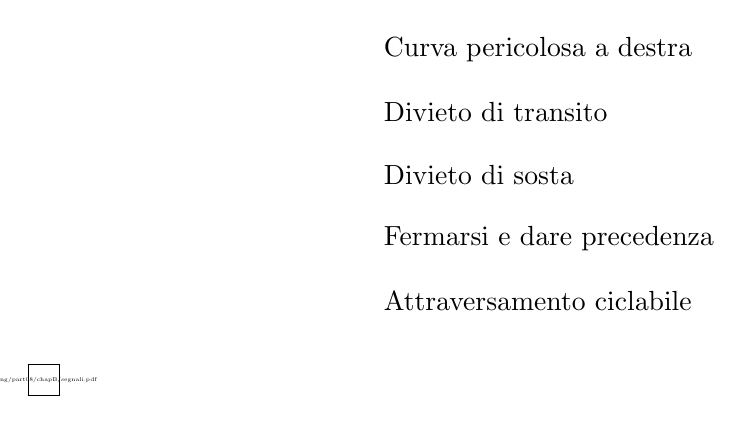
\begin{tikzpicture}[x=10mm, y=10mm, scale=.4]
    \pgftext[at=\pgfpoint {0mm}{0mm},left,base]{\pgfuseimage{segnali}};
    \node[right] (a) at (11,11) {Curva pericolosa a destra};
    \node[right] (b) at (11,9) {Divieto di transito};
    \node[right] (c) at (11,7) {Divieto di sosta};
    \node[right] (d) at (11,5) {Fermarsi e dare precedenza};
    \node[right] (e) at (11,3) {Attraversamento ciclabile};

\end{tikzpicture}
\end{center}
Traccia di soluzione:
\begin{itemize}
 \item se A e B partono insieme e arrivano insieme significa che hanno impiegato lo stesso tempo per fare il proprio viaggio;
 \item il tempo è dato dal rapporto tra lo spazio percorso e la velocità;
 \item la velocità di A è l'incognita del problema: la indichiamo con~$x$;
 \item l'equazione risolvente è~$\dfrac{110}{x}=\dfrac{132}{x+20}$.
\end{itemize}
Prosegui nella risoluzione.
\end{esercizio}

\begin{esercizio}
\label{ese:18.23}
Per percorrere~$480\unit{km}$ un treno impiega~$3$ ore di più di quanto impiegherebbe un aereo a percorrere~$\np[km]{1920}$.
L'aereo viaggia ad una velocità media che è~$8$ volte quella del treno. Qual è la velocità del treno?
\end{esercizio}
\newpage
\subsection{Risposte}

\paragraph{18.1.}
a)~$\{-3\}$;\quad b)~$\left\{\frac{3}{2}\right\}$;\quad c)~$\{0\}$;\quad d)~$\emptyset$.

\paragraph{18.2.}
a)~$\{0\}$;\quad b)~$\{-1\}$;\quad c)~$\left\{\frac{11}{6}\right\}$;\quad d)~$\emptyset$.

\paragraph{18.3.}
a)~$\emptyset$;\quad b)~$\insR-\{1\}$;\quad c)~$\emptyset$;\quad d)~$\{2\text{,~}-1\}$.

\paragraph{18.4.}
a)~$\left\{\frac{3}{2}\right\}$;\quad b)~$\{0\text{,~}-3\}$;\quad c)~$\{1\}$;\quad d)~$\{-2\}$.

\paragraph{18.5.}
a)~$\emptyset$;\quad b)~$\left\{\frac{9}{2}\right\}$;\quad c)~$\{-1\}$;\quad d)~$\left\{-{\frac{1}{3}}\right\}$.

\paragraph{18.6.}
a)~$\{-1\}$;\quad b)~$\left\{\frac{1}{3}\right\}$;\quad c)~$\emptyset$;\quad d)~$\{1\text{,~}-2\}$.

\paragraph{18.7.}
a)~$\left\{\frac{2}{25}\right\}$;\quad b)~$\emptyset$;\quad c)~$\emptyset$;\quad d)~$\left\{-{\frac{1}{3}}\right\}$.

\paragraph{18.8.}
a)~$\left\{\frac{3}{4}\right\}$;\quad b)~$\left\{\frac{7}{3}\right\}$;\quad c)~$\emptyset$;\quad d)~$\emptyset$.

\paragraph{18.9.}
a)~$\insR-\{2\}$;\quad b)~$\left\{-{\frac{3}{2}}\text{,~}\frac{5}{3}\right\}$;\quad c)~$\{-5\}$;\quad d)~$\{4\text{,~}-3\text{,~}3\}$.

\paragraph{18.10.}
a)~$\insR-\left\{-{\frac{2}{3}}\text{,~}2\right\}$;\quad b)~$\{1\}$;\quad c)~$\left\{-{\frac{2}{3}}\right\}$;\quad d)~$\{1\}$.

\paragraph{18.11.} %pag 180
a)~$\left\{-{\frac{1}{4}}\right\}$;\quad b)~$\emptyset$;\quad c)~$\emptyset$;\quad d)~$\{13\}$.

\paragraph{18.12.} %pag 472
a)~$\{0\}$;\quad b)~$\emptyset$;\quad c)~$\{1\}$;\quad d)~$\{6\}$.

\paragraph{18.13.}
a)~$\left\{\frac{1}{2}\right\}$;\quad b)~$\{2\text{,~}3\}$;\quad c)~$\left\{-\frac{2}{3}\right\}$;\quad d)~$\{2\}$.

\paragraph{18.14.}
a)~$\{-5,+1\}$;\quad b)~$\left\{2\text{,~}-\frac{1}{4}\text{,~}-2\right\}$;\quad c)~$\emptyset$;\quad d)~$\left\{-{\frac{3}{16}}\right\}$.

\paragraph{18.15.}
a)~$\insR-\{-3\}$;\quad b)~$\left\{\frac{3}{2}\right\}$;\quad c)~$\left\{\frac{35}{3}\right\}$;\quad d)~$\left\{-{\frac{3}{4}}\right\}$.

\paragraph{18.16.} %pag473
a)~$\{6\}$;\quad b)~$\{3\}$;\quad c)~$\left\{\frac{4}{3}\right\}$;\quad d)~$\{2\}$.

\paragraph{18.17.} %pag475
a)~$\emptyset$;\quad b)~$\left\{\frac{1}{3}\right\}$;\quad c)~$\left\{\frac{5}{8}\right\}$;\quad d)~$\left\{-{\frac{7}{8}}\right\}$.

\paragraph{18.18.}
a)~$\left\{\frac{5}{3}\right\}$;\quad b)~$\left\{-\frac{4}{3}\right\}$;\quad c)~$\{4\}$;\quad d)~$\left\{-{\frac{26}{25}}\right\}$;\quad e)~$\left\{\frac{12}{5}\right\}$;\quad f)~$\{-30\}$.

\paragraph{18.20.} $x=21$

\paragraph{18.21.} $x=28$
